\subsection{Interfaz Registrable}
Con el fin de agregar un nuevo experimento en la aplicaci�n, se debe crear una clase que herede de \textit{SingleObjectiveRegistrable} o \textit{MultiObjectiveRegistrable}, dependiendo de si el problema es monoobjetivo o multiobjetivo, respectivamente. La clases que heredan de \textit{Registrable} funcionan como \textit{templates} para crear nuevos experimentos. En la Figura \ref{fig:Registrable}, se presenta la jerarqu�a de clases de la interfaz \textit{Registrable}.

\begin{figure}[H]
    \centering
    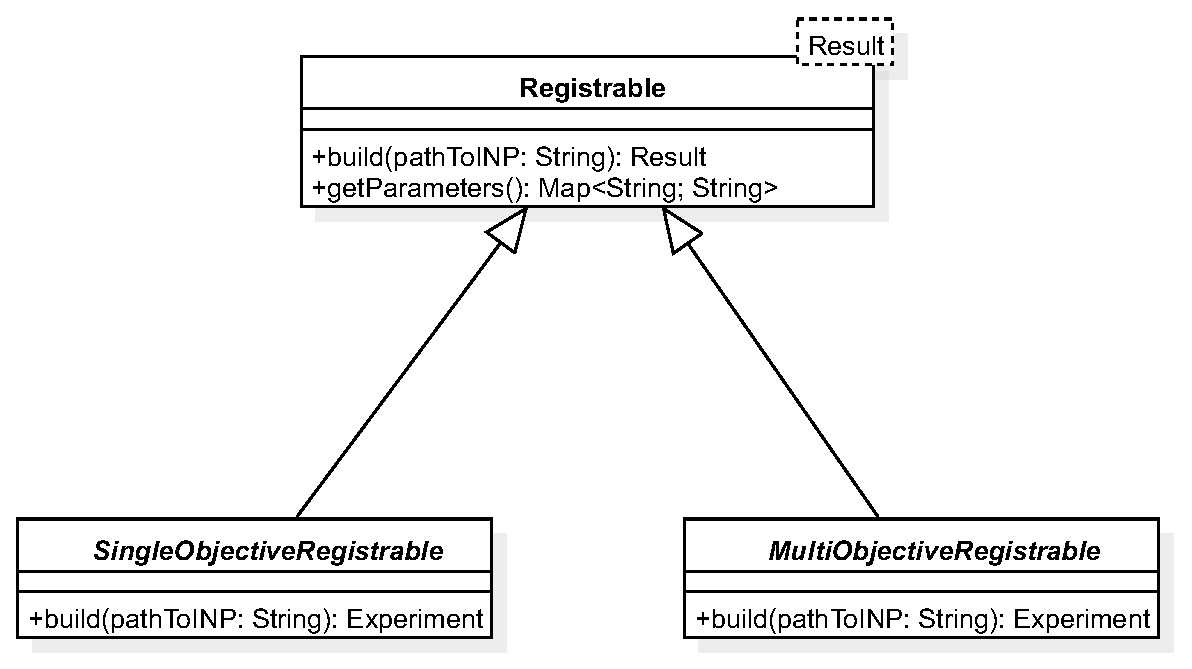
\includegraphics[width=\textwidth]{Seccion4/assets/d_class_registrable.eps}
    \caption{Jerarqu�a de clases de la interfaz Registrable.}
    \label{fig:Registrable}
\end{figure}
 
Ambas interfaces devuelven como resultado una instancia del experimento la cual es usada para realizar la simulaci�n. Los m�todos utilizados por la interfaz \textit{Registrable} son:
\begin{itemize}
    \item \textit{build}: Construye un experimento.
    \item \textit{getParameters}: Este m�todo devuelve un par clave valor, el cual es usado para agregar columnas extras a la ventana de resultados. La clave es usada como el nombre de la columna, mientras que el valor es usado como el valor de la columna. Este m�todo es opcional.
\end{itemize}

En el constructor p�blico de la clase que herede de una de las subinterfaces de \textit{Registrable}, se debe utilizar la anotaci�n \textit{@NewProblem}. Adicionalmente, si se quiere mostrar la interfaz de configuraci�n, dicho constructor debe incluir la anotaci�n \textit{@Parameters}.

Las clases que implementen cualquiera de las dos interfaces mencionadas anteriormente deben ser guardados en una estructura de datos, la cual es recorrida cuando se inicie la ejecuci�n del programa y analizada usando la \textit{Java Reflection API}. Este an�lisis consistir� en escanear y validar el cumplimiento de la convenci�n establecida para las clases que implementan est� interfaz. Esta convenci�n consiste en lo siguiente:
\begin{itemize}
    \item La clase debe contener un �nico constructor que use la anotaci�n @NewProblem.
    \item Si el constructor requiere par�metros �stos deben estar descritos usando la anotaci�n @Parameters.
    \item El constructor debe declarar los par�metros en el siguiente orden, de acuerdo con su tipo.
    \begin{enumerate}
        \item \textit{Object}: Usado para inyectar los operadores. Estos par�metros pueden posteriormente ser casteados a su tipo correcto. La anotaci�n correspondiente es \textit{@OperatorInput}.
        \item \textit{File}: Usados cuando el problema requiere informaci�n adicional que se encuentra en un archivo diferente. La anotaci�n correspondiente es \textit{@FileInput}.
        \item \textit{int}, \textit{Integer}, \textit{double} o \textit{Double}: Usado generalmente para configurar valores en el algoritmo o si el problema requiere otros valores que no fueron solicitados al crear los operadores. Las anotaciones correspondientes son \textit{@NumberInput} y \textit{@NumberToggleInput}.
        \item El constructor debe solicitar la misma cantidad de par�metros que las descritas en la anotaci�n \textit{@Parameters}.
    \end{enumerate}
\end{itemize}


Si estas convenciones no se cumplen, entonces un error en tiempo de compilaci�n ser� emitido. 

El orden en el que son inyectados los par�metros consiste en el siguiente:

\begin{enumerate}
    \item Par�metros descritos por \textit{@OperatorInput}.
    \item Par�metros descritos por \textit{@FileInput}.
    \item Par�metros descritos por \textit{@NumberInput}.
    \item Par�metros descritos por \textit{@NumberToggleInput}.
\end{enumerate}

Una vez que se haya configurado el problema a trav�s de la interfaz, se crear� la instancia de la clase que hereda de \textit{Registrable} y se llamar� a su m�todo \textit{build}, para crear el experimento y comenzar su ejecuci�n.

La estructura de datos para registrar las clases que heredan de \textit{SingleObjectiveRegistrable} y \textit{MonoObjectiveRegistrable} se encontrar� en la clase \textit{RegistrableConfiguration}.

En las Figura \ref{fig:constructor_registrable}, \ref{fig:build_registrable}, \ref{fig:getParameters_registrable}, se muestran un ejemplo del constructor, uno del m�todo \textit{build} y uno del m�todo \textit{getParameters}, utilizado en el problema de optimizaci�n de los costos de las tuber�as.
 
\begin{figure}[H]
    \centering
    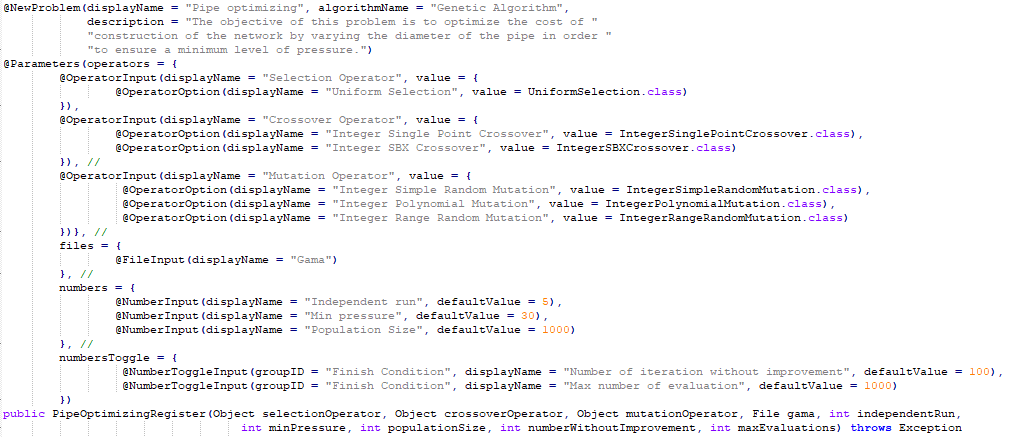
\includegraphics[width=\textwidth]{Seccion4/assets/ConstructorHeredadoRegistrable.png}
    \caption{Constructor de la clase \textit{PipeOptimizingRegister}.}
    \label{fig:constructor_registrable}
\end{figure}

\begin{figure}[H]
    \centering
    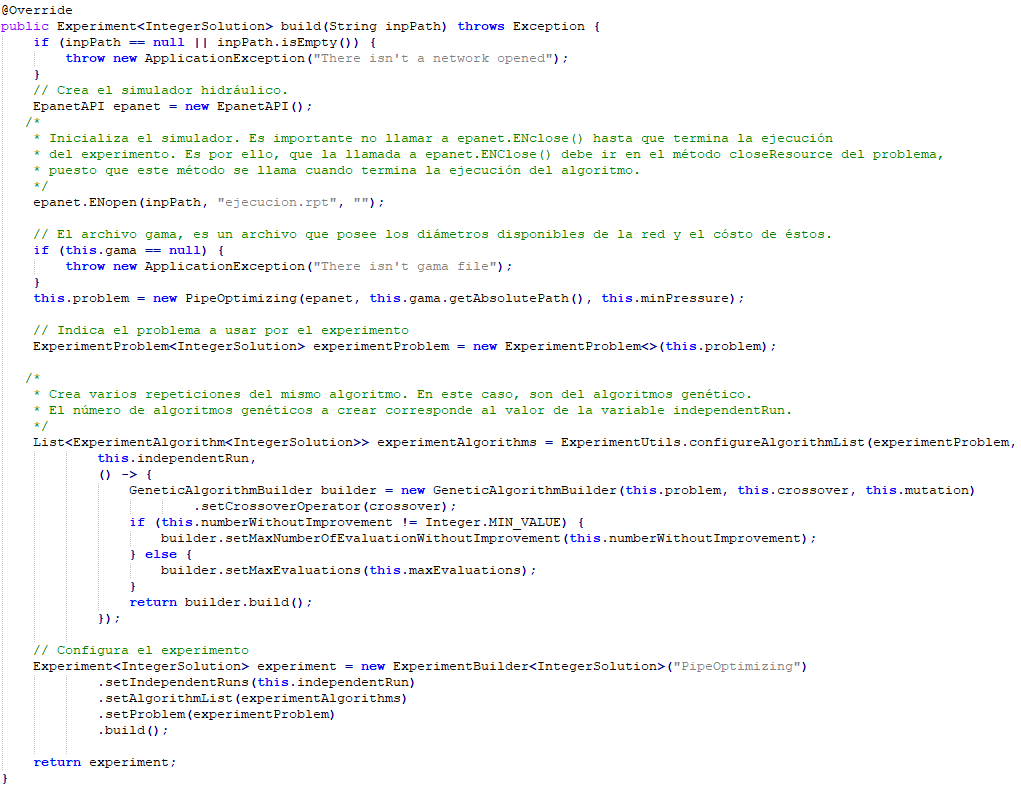
\includegraphics[width=\textwidth]{Seccion4/assets/BuildMethodPipeOptimizingRegister.png}
    \caption{Implementaci�n del m�todo build de la clase \textit{PipeOptimizingRegister}.}
    \label{fig:build_registrable}
\end{figure}

\begin{figure}[H]
    \centering
    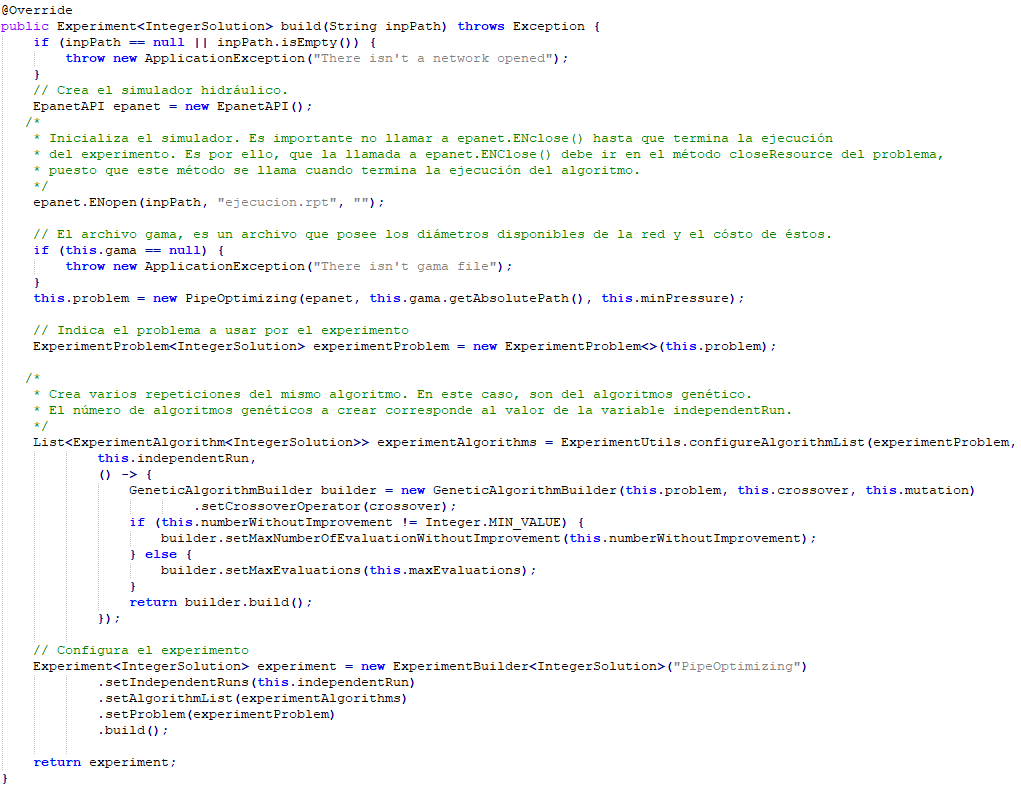
\includegraphics[width=\textwidth]{Seccion4/assets/BuildMethodPipeOptimizingRegister.png}
    \caption{Implementaci�n del m�todo opcional getParameters de la clase \textit{PipeOptimizingRegister}.}
    \label{fig:getParameters_registrable}
\end{figure}

